% Template for PLoS
% Version 3.3 June 2016
%
% % % % % % % % % % % % % % % % % % % % % %
%
% -- IMPORTANT NOTE
%
% This template contains comments intended 
% to minimize problems and delays during our production 
% process. Please follow the template instructions
% whenever possible.
%
% % % % % % % % % % % % % % % % % % % % % % % 
%
% Once your paper is accepted for publication, 
% PLEASE REMOVE ALL TRACKED CHANGES in this file 
% and leave only the final text of your manuscript. 
% PLOS recommends the use of latexdiff to track changes during review, as this will help to maintain a clean tex file.
% Visit https://www.ctan.org/pkg/latexdiff?lang=en for info or contact us at latex@plos.org.
%
%
% There are no restrictions on package use within the LaTeX files except that 
% no packages listed in the template may be deleted.
%
% Please do not include colors or graphics in the text.
%
% The manuscript LaTeX source should be contained within a single file (do not use \input, \externaldocument, or similar commands).
%
% % % % % % % % % % % % % % % % % % % % % % %
%
% -- FIGURES AND TABLES
%
% Please include tables/figure captions directly after the paragraph where they are first cited in the text.
%
% DO NOT INCLUDE GRAPHICS IN YOUR MANUSCRIPT
% - Figures should be uploaded separately from your manuscript file. 
% - Figures generated using LaTeX should be extracted and removed from the PDF before submission. 
% - Figures containing multiple panels/subfigures must be combined into one image file before submission.
% For figure citations, please use "Fig" instead of "Figure".
% See http://journals.plos.org/plosone/s/figures for PLOS figure guidelines.
%
% Tables should be cell-based and may not contain:
% - spacing/line breaks within cells to alter layout or alignment
% - do not nest tabular environments (no tabular environments within tabular environments)
% - no graphics or colored text (cell background color/shading OK)
% See http://journals.plos.org/plosone/s/tables for table guidelines.
%
% For tables that exceed the width of the text column, use the adjustwidth environment as illustrated in the example table in text below.
%
% % % % % % % % % % % % % % % % % % % % % % % %
%
% -- EQUATIONS, MATH SYMBOLS, SUBSCRIPTS, AND SUPERSCRIPTS
%
% IMPORTANT
% Below are a few tips to help format your equations and other special characters according to our specifications. For more tips to help reduce the possibility of formatting errors during conversion, please see our LaTeX guidelines at http://journals.plos.org/plosone/s/latex
%
% For inline equations, please be sure to include all portions of an equation in the math environment.  For example, x$^2$ is incorrect; this should be formatted as $x^2$ (or $\mathrm{x}^2$ if the romanized font is desired).
%
% Do not include text that is not math in the math environment. For example, CO2 should be written as CO\textsubscript{2} instead of CO$_2$.
%
% Please add line breaks to long display equations when possible in order to fit size of the column. 
%
% For inline equations, please do not include punctuation (commas, etc) within the math environment unless this is part of the equation.
%
% When adding superscript or subscripts outside of brackets/braces, please group using {}.  For example, change "[U(D,E,\gamma)]^2" to "{[U(D,E,\gamma)]}^2". 
%
% Do not use \cal for caligraphic font.  Instead, use \mathcal{}
%
% % % % % % % % % % % % % % % % % % % % % % % % 
%
% Please contact latex@plos.org with any questions.
%
% % % % % % % % % % % % % % % % % % % % % % % %

\documentclass[10pt,letterpaper]{article}
\usepackage[top=0.85in,left=2.75in,footskip=0.75in]{geometry}

% amsmath and amssymb packages, useful for mathematical formulas and symbols
\usepackage{amsmath,amssymb}

% Use adjustwidth environment to exceed column width (see example table in text)
\usepackage{changepage}

% Use Unicode characters when possible
\usepackage[utf8x]{inputenc}

% textcomp package and marvosym package for additional characters
\usepackage{textcomp,marvosym}

% cite package, to clean up citations in the main text. Do not remove.
\usepackage{cite}

% Use nameref to cite supporting information files (see Supporting Information section for more info)
\usepackage{nameref,hyperref}

% line numbers
\usepackage[right]{lineno}

% ligatures disabled
\usepackage{microtype}
\DisableLigatures[f]{encoding = *, family = * }

% color can be used to apply background shading to table cells only
\usepackage[table]{xcolor}

% array package and thick rules for tables
\usepackage{array}

% create "+" rule type for thick vertical lines
\newcolumntype{+}{!{\vrule width 2pt}}

% create \thickcline for thick horizontal lines of variable length
\newlength\savedwidth
\newcommand\thickcline[1]{%
  \noalign{\global\savedwidth\arrayrulewidth\global\arrayrulewidth 2pt}%
  \cline{#1}%
  \noalign{\vskip\arrayrulewidth}%
  \noalign{\global\arrayrulewidth\savedwidth}%
}

% \thickhline command for thick horizontal lines that span the table
\newcommand\thickhline{\noalign{\global\savedwidth\arrayrulewidth\global\arrayrulewidth 2pt}%
\hline
\noalign{\global\arrayrulewidth\savedwidth}}


% Remove comment for double spacing
%\usepackage{setspace} 
%\doublespacing

% Text layout
\raggedright
\setlength{\parindent}{0.5cm}
\textwidth 5.25in 
\textheight 8.75in

% Bold the 'Figure #' in the caption and separate it from the title/caption with a period
% Captions will be left justified
\usepackage[aboveskip=1pt,labelfont=bf,labelsep=period,justification=raggedright,singlelinecheck=off]{caption}
\renewcommand{\figurename}{Fig}

% Use the PLoS provided BiBTeX style
\bibliographystyle{plos2015}

% Remove brackets from numbering in List of References
\makeatletter
\renewcommand{\@biblabel}[1]{\quad#1.}
\makeatother

% Leave date blank
\date{}

% Header and Footer with logo
\usepackage{lastpage,fancyhdr,graphicx}
\usepackage{epstopdf}
\pagestyle{myheadings}
\pagestyle{fancy}
\fancyhf{}
\setlength{\headheight}{27.023pt}
\lhead{
\includegraphics[width=2.0in]{PLOS-submission.eps}}
\rfoot{\thepage/\pageref{LastPage}}
\renewcommand{\footrule}{\hrule height 2pt \vspace{2mm}}
\fancyheadoffset[L]{2.25in}
\fancyfootoffset[L]{2.25in}
\lfoot{\sf PLOS}

%% Include all macros below

\newcommand{\cursedforest}{{\sc CursedForest}}
\newcommand{\mtry}{{\texttt mtry}}
\newcommand{\ntree}{{\texttt ntree}}

%% END MACROS SECTION

%% Additional packages
\usepackage{footmisc}
\usepackage{multirow}


%%local edits (rob)
\let\oldmarginpar\marginpar
\renewcommand\marginpar[1]{\-\oldmarginpar[\raggedleft\footnotesize #1]%hv
{\raggedright\footnotesize #1}}
\reversemarginpar
\setlength{\marginparwidth}{5cm}


\begin{document}
\vspace*{0.2in}

% Title must be 250 characters or less.
\begin{flushleft}
{\Large
\textbf\newline{\cursedforest\ - A Random Forest Implementation for ``Big'' and ``Wide'' Data} % Please use "title case" (capitalize all terms in the title except conjunctions, prepositions, and articles).
}
\newline
% Insert author names, affiliations and corresponding author email (do not include titles, positions, or degrees).
\\
Aidan O'Brien\textsuperscript{1},
Piotr Szul\textsuperscript{2},
Stephanie Li\textsuperscript{3},
James Doecke\textsuperscript{3},
Nick Ellis\textsuperscript{4},
Robert Dunne\textsuperscript{5}, and
Denis C. Bauer\textsuperscript{1,*}
%, with the Lorem Ipsum Consortium\textsuperscript{\textpilcrow}
\\
\bigskip
\textbf{1} Health \& Biosecurity, CSIRO, Sydney, NSW, Australia
\\
\textbf{2} Data61, CSIRO, Brisbane, QLD, Australia
\\
\textbf{3} Health \& Biosecurity, CSIRO, Brisbane, QLD, Australia
\\
\textbf{4} Oceans \& Atmosphere, CSIRO, Brisbane, QLD, Australia
\\
\textbf{5} Data61, CSIRO, Sydney, NSW, Australia
\\
\bigskip

% Insert additional author notes using the symbols described below. Insert symbol callouts after author names as necessary.
% 
% Remove or comment out the author notes below if they aren't used.
%
% Primary Equal Contribution Note
%\Yinyang These authors contributed equally to this work.

% Additional Equal Contribution Note
% Also use this double-dagger symbol for special authorship notes, such as senior authorship.
%\ddag These authors also contributed equally to this work.

% Current address notes
%\textcurrency a Insert current address of first author with an address update
% \textcurrency b Insert current address of second author with an address update
% \textcurrency c Insert current address of third author with an address update

% Deceased author note
%\dag Deceased

% Group/Consortium Author Note
%\textpilcrow Membership list can be found in the Acknowledgments section.

% Use the asterisk to denote corresponding authorship and provide email address in note below.
* Denis.Bauer@CSIRO.au

\end{flushleft}
\tableofcontents
\clearpage
\section{Notes}
\begin{itemize}
\item I think the structure of the first section should be
  \begin{itemize}
  \item convergence results from Biau 2012  (done)
  \item consider  \cite{Segal.2004} examples
  \item simulations reproduced from Genuer et al 2010 (no -- we need classification examples)
  \item check Piotr's simulation  (done)
  \item run spark ML or CursedForest on the  simulation data 
  \item we extend the simulations to many more variables 
  \item I dont think I can get R to handle chromosme 1 etc. May have to run CF on chromosme 22, see table
    \ref{table:smaller_data} -- On it, Aidan
  \item variable  selection may succeed where accurate prediction does not
  \item discussion of the effect of the \ntree\ and \mtry\ parameters for variable selection with many noise variables
  \item   perhaps we argue that in the case where the relationship of $X$ and $y$ takes a particular form (step, ramp) we can recover
    the significant variables in the presence of a very large number of noise variables
  \item in the case of genomic data, our functions of interest are more likely to be stop or ramp functions rather than harmonic
    functions. So we have some hope.
  \end{itemize}
\item check out 
  \begin{itemize}
  \item D\'iaz-Uriarte, R., \& Alvarez de Andr\'es, S. (2006). (done)
  \item \cite{Goldstein.et.al.2011}
notes that the 0, 1, 2 encoding of alleles is an additive model i.e. each additional minor allele increases the effect 
\begin{verbatim}
Different genetic effects
Type	Mechanism	Partition
Additive	Each additional minor allele increases variation	0, 1, 2
Dominant	Presence of at least 1 minor allele increases variation	0, 1/2
Recessive	Two minor alleles needed for variation	0/1, 2
Heterosis	Heterozygote leads to variation	0/2, 1
\end{verbatim}

  \item Chen (2012)  (done)
  \item VSURF and  varSelRF, (done) recursive feature (forwards backwards) using variable importance
  \item \cite{Wright.and.Ziegle.2016} ranger package (doing it!)
  \item  r2VIM: A new variable selection method for random forests in
    genome-wide association studies
  \item CloudForest: A Scalable and Efficient Random Forest
    Implementation for Biological Data
   Ensembles of decision trees in go/golang   --  do we need to look
   at this? 
  \item \cite{Tuv.et.al.2009} feature selection via adding permuted variables. Do we want to consider this? (no, leave it for now)
  \end{itemize}
\item other things to do
  \begin{itemize}
  \item what is the problem with bagging? Do we need to redo the thousand genome stuff?
  \end{itemize}
\end{itemize}


\clearpage

% Please keep the abstract below 300 words
\section{Abstract}
The abstract.

\linenumbers

\section{Introduction}

The digital revolution is seeing a dramatic increase in data collected about every aspect of life~\cite{Loebbecke2015}.
These data sets are not only growing vertically, by capturing more events, but also horizontally by capturing
more information about these events.  The challenge of big and ``wide'' data is especially pronounced in the health
space where, for example, whole genome sequence (WGS) technology enables researchers to interrogate all 3 billion base pairs of the
human genome.

Identifying the relevant and disease specific base-pair difference between individuals is the focus of genome wide
association studies (GWAs).  These analysis are typically performed on only the most frequently differing base-pairs
(SNPs) by applying linear or logistic regression analysis to each SNP separately~\cite{CCC2007}.  It has since been
demonstrated that not taking joint interactions between SNPs into account when filtering for potential disease mutations
is inadequate~\cite{Manolio2009}.  
Complex trait analysis has demonstrated that in order to explain the overall
heritability a model needs to take the joint contribution of all variants into account~\cite{Yang2011}.


\marginpar{decison trees capture interaction -- there is no main effect term. Random forests inherit this property. I dont think it
  has anything to do with boostrapping, the point of which is to ensure that successive trees are not correlated.}
Random forests~\cite{Breiman2001} are able to capture interactions between features while still allowing to
prioritise SNPs for their contribution to disease.  The joint interaction is achieved by applying the technique of
bootstrap aggregation or bagging to decision trees, while a measure of variable importance can be provided, for example,
by summing the number of times a variable is used to split a node, over all nodes and all trees.  Random forests are well suited for
processing ``wide'' genomic data for two reasons.  Firstly, while other machine learning applications have the
propensity to overfit datasets with more features $p$ than samples $n$ (a consequence of the ``curse of
dimensionality''~\cite{Bauer2014, bellman1961adaptive}), decision trees are resistant to overfitting. 
Secondly, random forests are also very easy to parallelise. As the forest is a sum of decision trees, it it possible to grow
separate trees on different processors and combine the trees.

The most popular random forest software packages are R-based, although current implementations do not scale well with
increasing feature size~\cite{Wright.and.Ziegle.2016}.  This is despite R now supporting long vectors (length greater
than $2^{31}$), and the {\sc randomForest} implementation in R lending itself to parallelization to grow multiple trees
simultaneously~\cite{Liaw.and.Weiner.2002} and them combine them.  More suitable implementations for ``wide'' genomic data have been
developed in other programming languages.  {\sc CloudForest}~\cite{Bressler2015} written in Go, achieves fast running
times by effective use of the CPU cache, optimising for different classes of features and efficiently multi-threading.
Similarly, {\sc Ranger}~\cite{Wright.and.Ziegle.2016} written in C++ with an R front-end is specifically optimised for
dealing with large data sets.

However, the use of traditional compute infrastructure limits the parallelization strategies that can be employed by
these methods.  The programs are limited to utilising only CPUs that are on the same computer node (multi-threading) or
else they run on CPUs distributed across nodes by virtue of the fact that there is no communication between the
processes (a separate tree is grown on each node).  Hadoop/Spark overcomes these limitation by enabling programs to
scale beyond compute-node boundaries and hence enable more sophisticated parallelization strategies.  In the case of
random forests this means that the computations for each node of a tree can be handed off to separate processors.
  
Here we introduce \cursedforest, a Hadoop/Spark based implementation of random forests specifically designed to cater for
``big'' (many samples) and ``wide'' (many features) data sets. \cursedforest\ is capable of parallelising the split for
each node in a tree thereby handling millions of features, such as in the 1000 Genomes Project data, which consists
of approximately 2500 samples with up to 80 million variants~\cite{1KG2012}.  By also utilising Spark to read in and
manipulate the standard genomic variant format (VCF) directly, \cursedforest\ outperforms existing tools even on small
datasets where multi-threading generally performs well. 
 \marginpar{Piotr this is your 20 trees has the important
  feature in the top 5 and 100 trees has it always as the top element, do we need to spell this out better, it should be
  a result section.}
Harnessing the virtually unlimited capability to parallelise tasks, \cursedforest\ can build a large number of trees,
which boosts the accuracy for variable importance selection~\cite{Szymczak2016}.

\cursedforest\ is included in our previously developed framework for Spark-based genomic data analysis,
VariantSpark~\cite{OBrien2015}, which therefore now enables supervised and unsupervised machine learning. This offers a
comprehensive analysis toolkit that can scale for the future data demands, where the richness from WGS data can be
utilised to ``fill in'' or impute the information at previously unobserved genomic positions in older array
technology~\cite{Howie2012}.  This provides the potential to impute samples in the GWAs catalogue and generate datasets
of hundreds of thousands of individuals with millions of variants, highlighting the need for incorporating modern
compute paradigms to deal with these challenges.

A Spark application runs on a ``driver'' node and distributes tasks to the many ``worker'' nodes, or ``executors''.

We previously demonstrated the versatility and scalability of Spark by developing VariantSpark~\cite{OBrien2015}, a
framework allowing users to easily analyse Variant Call Format (VCF) files using ML algorithms on the Spark framework.
Using VariantSpark, we successfully built a k-means model on the full $2500 \times 80$ million matrix to cluster
individuals by their ethnicity achieving an Adjusted Rand Index of 0.84 (with 1 being perfect clustering and -1 random
clustering).

Here we extend this toolkit to encompass supervised learning using random forests.  Spark ML's random forest implementation is not
able to handle the extremely ``wide'' genomic data as it was developed for large number of samples with only modest
dimensionality.  Although Spark ML can build a random forest model on a subset of the data (chromosome 1~and~2), the time taken is
excessive due to the huge amount of data being aggregated and processed by the single driver node during intermediate
stages of building the model (see Result~\ref{comp}).  This unbalanced work load where the driver node becomes the
bottleneck and worker nodes being idle prevents a seamless scaling to larger datasets. The memory requirements per
executor also increases with dimensionality due to the data types Spark ML uses, which we elaborate on in the
discussion.

%% We therefore developed \cursedforest\, a Spark-based random forest algorithm able to process big and ``wide'' data.
%% % Unlike the standard Apache implementation, \cursedforest\ is able to easily process data with millions of dimensions without
%% % excessive resource requirements on the driver or worker nodes.  DENIS Piotr this is your 20 trees has the important feature in
%% % the top 5 and 100 trees has it always as the top element, do we need to spell this out better, it should be a result section.
%% \marginpar{Piotr this is your 20 trees has the important feature in the top 5 and 100 trees has it always as the top
%%   element, do we need to spell this out better, it should be a result section.}  Harnessing the virtually unlimited
%% capability to parallelise tasks, \cursedforest\ can build a large number of trees, which boosts the accuracy for
%% variable selection as demonstrated by {\sc r2VIM}~\cite{Szymczak2016} on smaller datasets.
 

%Hadoop/Spark overcomes this limitation by enabling programs to scale beyond compute-node boundaries and virtually utilise infinite number of CPUs.   
%Therefore, these historically successful solutions are not catering for the big data demands that especially due to WGS are becoming more prevalent. Here, classification or feature importance analysis needs to be performed on datasets with a much larger number of features~\cite{Yano2016}. 
%For example, the 1000 Genome data consists of approximately 2500 samples with up to 80 million variants~\cite{1KG2012},
%This dataset consumes close to a terabyte of disk space.  
%We previously demonstrated the versatility and scalability of Spark by developing VariantSpark~\cite{OBrien2015}, a
%framework allowing users to easily analyse Variant Call Format (VCF) files using ML algorithms on the Spark framework.
%Using VariantSpark, we successfully built a k-means model on the full
%$2500 \times 80$ million matrix to cluster individuals by
%their ethnicity achieving an Adjusted Rand Index of 0.84 (with 1 being perfect clustering and -1 random clustering).

%Spark ML's random forest implementation is not able to handle the extremely ``wide'' genomic data as it was developed for large number of samples with only modest dimensionality.  
%Although Spark ML can build a random forest model on
%a subset of the data (chromosome 1~and~2), the time taken is excessive due to the huge amount of data being aggregated
%and processed by the single driver node during intermediate stages of building the model (see Result~\ref{comp}).  This
%unbalanced work load where the driver node becomes the bottleneck and worker nodes being idle prevents a seamless
%scaling to larger datasets. The memory requirements per executor also increases with dimensionality due to the data types
%Spark ML uses, which we elaborate on in the discussion.
%
%We therefore developed \cursedforest\, a Spark-based random forest algorithm able to process big and ``wide'' data. 
%Unlike
%the standard Apache implementation, \cursedforest\ is able to easily process data with millions of dimensions without
%excessive resource requirements on the driver or worker nodes.
%DENIS Piotr this is your 20 trees has the important feature in the top 5 and 100 trees has it always as the top element, do we need to spell this out better, it should be a result section.


\marginpar{Needs to be rewritten once we actually have the sections} 
In the first section we explore some of the
properties of random forests, demonstrating that any potential flaws in \cursedforest\ are an inherent property of random
forests. Here we provide demonstrations using synthetic data.  We then demonstrate the scalability of \cursedforest\ in
respect to the dimensionality of the data, building a random forest model on whole-genome data from the 1000 Genomes Project. Here
we report on the accuracy (in terms of the ARI)
\marginpar{what is ARI?}
 and the error.  Finally, given the role different parameter values can
play in model construction, we explore the effect tuning these parameters can have on the prediction accuracy of the
model.



\section{Methods}

%%%%%%%%%%%%%%%%%%%%%%%%%%%%%%%%%%%%%%%%%%%%
\marginpar{Rob can you condense this down into what is relevant for this paper and not explained elsewhere in the literature}
\subsection{Overview of Random Forests}

Decision trees have a number of desirable features, they:
\begin{itemize}
  \item are invariant to monotonic scaling of the data;
  \item can handle categorical and real valued inputs;
  \item can handle missing values;
  \item are insensitive to useless predictors;
  \item are able to capture interactions between features (which is of importance for modelling complex polygenic diseases).
  \end{itemize}
However, the tree fitting algorithm is greedy and may generate an unstable model. That is, a small change in the data may
lead to a very different model. 

Random forests~\cite{Breiman2001} (RFs) apply the technique of bootstrap aggregation or bagging to decision trees.  The training
data is independently drawn from the joint distribution of $(X,Y)$ and comprises $n$ $(p+1)$-tuples $(x_1,y_1),\ldots, (x_n,y_n)$.
$X$ and $\theta_b$ for $b=1,\ldots,B$ are i.i.d. random vectors and a tree is grown on each of these $\theta_b$ samples 
($X$ is randomly sampled $B$ times with replacement and a tree is grown on each of these $B$ samples). 
The results are combined in an appropriate way. In a classification problem we take the majority vote for the trees over
the $q=1,..,Q$ classes,
\begin{equation*}
{{h_f}}= \arg \max_q \left(\sum_b I(h(x;\theta_b)=q)\right).
\end{equation*}

Random forests are a variance reduction technique. They take unpruned tree models, which have a low bias but a high
variance, and by combining them reduce the variance. As the prediction error is the sum of the variance and the bias
squared, this strategy should lead to a low prediction error.

The average prediction error for an individual tree $h(X; \theta)$ is
\begin{equation}
PE_t = E_\theta E_{X,Y} (Y-h(X; \theta))^2.
\end{equation}
Assume that, for all $\theta$, the tree is unbiased, i.e., $EY= E_X h(X; \theta)$. Then
\begin{equation}
PE_f \leq \rho PE_t
\end{equation}
where $\rho$ is the weighted correlation between residuals $(Y-h(X;\theta))$ and $(Y-h(X;\theta^\prime))$ for independent $\theta,
\theta^\prime$.  
So what is required for accurate random forest regression is (i) low correlation between residuals of differing tree in
the forest, and (ii) low prediction error for the individual trees \cite{Segal.2004}. In addition to growing the trees
on bootstrapped samples, each node in the tree is split on a randomly selected subset of the variables.

The benefits of random forest models are:
  \begin{itemize}
  \item they give an out-of-bag estimate of model accuracy, by using the samples not selected for the bootstrapped sample
    as an independent test set for each tree;
  \item they provide a measure of variable importance, for example by summing the number of times a variable is used to
    split a node, over all nodes and all trees. More complex measures of variable importance are also used;
  \item they inherit some of the qualities of tree models (but not, for example, the handling of missing values via surrogate
    variables. This would be difficult as the trees as split on random subsets of variables).
  \end{itemize}

Since the original implementation of random forests, there have been a number of developments leading to a better understanding of
the algorithm. 
\begin{itemize}
\item random forests are resistant to overfitting. However it is not true that they will not overfit,
  ~\cite{Segal.2004} gives examples of overfitting in the case where:
  \begin{itemize}
  \item a single tree is the most appropriate model; and
  \item the variables are highly correlated so that the bootstrap resampling does not give rise to uncorrelated trees.
  \end{itemize}
However, keeping these difficult cases in mind, random forests have a strong claim to being resistant to overfitting.

\item \cite{Strobl.et.al.2007} demonstrates that the random forest algorithm is subject to a bias in variable selection via two mechanisms:
  \begin{enumerate}
  \item differences in variable scale (for $X_i$ continuous) and number of levels (for $X_i$ discrete) introduces a
    bias. A uninformative variable with a large number of levels may be selected over a more informative variable with
    fewer levels;
  \item bagging introduces a bias, but sampling $(1- 1/e) \approx 0.632$ of the data without replacement seems to be an
    effective strategy for removing the problem.
  \end{enumerate}
\end{itemize} 

\cite{Strobl.et.al.2007} introduce changes to the random forest algorithm to fix 1) and 2).  However the level effect will be
apparent in the CF algorithm as well.  However, there are many examples, particularly in genomics, where we have data
sets that are
\begin{itemize}
\item very wide;
\item all variables have the same number of levels (for example, measurements at different points along the genome);
\item the hypothesized functional relationship is of a form amenable to a decision tree.
\end{itemize}

\subsubsection{convergence}
Biau {\it et al.}~\cite{Biau.2012} provide a proof that a random forest model will converge at a rate that depends on
the cardinality of the set $S$ of ``strong predictors'' rather than on the number of variables $p$. That is, given a
function $y=f(S)$ depending on a set of variables $S$, a random forest will converge to the true function $y$ with a
rate that depends on the size of $S$ and not the number of noise variables in the data set. If the size of $S$ is small
compared to the total number of variables, then the rate of convergence will be quicker.
\marginpar{say something about the rate of convergence}

Subject to certain conditions, random forests will not overfit even in the $p > n$ case. 
Here we demonstrate that this may hold true in extreme cases where $p \gg n$.

\marginpar{why is this relevant, i.e. if this is special to VariantSpark it should be explained better.}
\subsubsection{variable selection}
\cite{Genuer.et.al.2010} and \cite{Diaz.and.Alvarez.2006} describe iterative schemes for doing variable selection using
the importance measure. See \cite{Chen.and.Ishwaran.2012} for a review of the area with particular reference to genomic
data.
\marginpar{ \cite{Chen.and.Ishwaran.2012} cite many papers on extensions of random forests to handle 
GWAS data. What do we need to do in this area? What about linkage diseqelibrium?}


%%%%%%%%%%%%%%%%%%%%%%%%%%%%%%%%%%%%%%%%%%%%%%%%%%%%%%%%%%%
\subsection{\cursedforest.}
% DENIS: Aidan and Piotr can you please explain here how CursedForest is implemented
Traditionally, VariantSpark made use of Spark's machine learning algorithms ``Spark ML''. These algorithms require data
in a ``DataFrame'', similar to DataFrames in R.

Traditionally, VariantSpark used the random forest algorithm from Spark ML. While Spark ML algorithms demonstrate
scalability when dealing with a large number of samples, this scalability quickly breaks down as we include more
features.

One of the restrictions preventing Spark ML algorithms from scaling to high-dimensionality data is that the feature-set
for each sample is stored as a vector data type. Spark vectors are stored in resilient distributed dataset (RDDs), and
while RDDs can be split, vectors cannot. So as we add more samples (in our case individuals), Spark ML can simply split
the RDD into more partitions and resource requirements will remain relatively stable. However, as the number of
dimensions (variants) increases, the size of the vectors increases. This results in higher memory-requirements as
increasingly large vectors must be loaded into memory.

On the other hand, \cursedforest\ (CF) is specifically designed to handle wide ``cursed'' data. It avoids the relation
between memory and dimensionality by avoiding calculations that rely on entire feature vectors.

Compared to Spark ML, \cursedforest\ further parallelizes work down to individual features.  For example, for each node of
a tree, \cursedforest\ will distribute tasks that consist of single features (variants), for every individual.  Each of
these tasks will calculate the information gain for that specific feature.  Once these tasks have completed, the results
are reduced to return the feature which gives the greatest information gain.  This process is then repeated until
\cursedforest\ has created the entire decision tree.

The current implementation of \cursedforest\ uses:
\begin{itemize}
\item an ``information gained'' criteria for splitting. Let $f_q$ be the fraction of items labelled with value $q$ where $q = 1,
  \ldots, Q$ at a node. The entropy of the node is $H = - \sum^{m}_{i=1} f_i \log^{}_2 f_i.$
The expected information gain is the change in entropy $H$ from a prior state $T$ to a state that takes some
information $a$ as given: 
\[ IG(T,a) = H(T) - H(T|a). \]
In this case, the information gain is IG = Entropy(parent node) - Weighted Sum of Entropy(Children)
\item variable importance is the sum of IG over all notes and all trees for that variable
\end{itemize}


%%%%%%%%%%%%%%%%%%%%%%%%%%%%%%%%
% This section talks about the datasets
%%%%%%%%%%%%%%%%%%%%%%%%%%%%%%%%
\subsection{Datasets}
\subsubsection{1000 Genomes Project}
We obtained the 1000 Genomes Project data as VCF files from their FTP site.  Each VCF file contains the variants for every individual accross one chromosome.  
We use the phase 3 dataset which contains 2,504 individuals with approximately 81 million variant positions (i.e. a matrix of $2,504 \times 81$ million).  
For compatibility with the majority of the algorithms we demonstrate, we convert the original variant representations to double representations.  
For example, we store the absence of a variant (0\textbar0) as 0.0, a heterozygous variant (1\textbar0 or 0\textbar1)as 1.0. and a homozygous variant (1\textbar1) as 2.0.

\subsubsection{The Cancer Genome Atlas}
We obtained The Cancer Genome Atlas (TCGA) BRCA data as VCF files from the GDC data portal.
This data is in the category ``Simple Nucleotide Variation''.
After downloading, we use a custom script to name the samples in the files and filter for only the "Normal" tissue column.
We then use GATK to merge the files into a single VCF file.

%DENIS: Rob how was the synthetic data generated
\subsubsection{Synthetic data} 
Each dataset consists of $n$ samples and $m$ variables where $n << m$, and values for each variable are ordinal factors with
three levels represented as numbers $\{0, 1, 2\}$ (which correspond to an additive effect encoding of genomics variation) randomly
generated from uniform distribution with equal probabilities.  The dichotomous response is generated from a two level
Bernoulli trail with $p$ (probability of success) calculated by applying inverse logit transformation to the continuous
linear response ($y$) of five variables:
$$y = a_{10}* v_{10} + a_{100}*v_{100} + a_{1000}*v_{1000} + a_{10000}*v_{10000} + a_{10000}*v_{100000}$$
where $a_{10} = 0.8, a_{100} = 0.9, a_{1000} = 1.1, a_{10000} = 1.0, a_{10000}=1.15$.



\subsection{Parameter settings}
We consider the parameter setting for the random forest algorithm. We use the R terms from the {\sc randomForest} package
\cite{Liaw.and.Weiner.2002} which incorporates the original Fortran code by Brieman and Cutler.  We incorporate the
advice of \cite{Liaw.and.Weiner.2002}, which we have found mirrors our own experience.

\begin{itemize}
\item \ntree\ the number of trees.  The number of trees necessary for good performance grows with the number of predictors.
  \marginpar{can we do proximity?} \cite{Liaw.and.Weiner.2002} suggest that a high \ntree\ is necessary to get stable
  estimates of variable importance and proximity; however, even though the variable importance measures may vary from run to run,
  the ranking of the importances is quite stable.  In addition, we note that it is possible for a random forest model to have a very poor
  fit, and be useless for prediction, and still have a useful ranking of variable importance.
\item \mtry\ -- the number of variables considered at each split (if \mtry=$p$, we have a boosted decision
  tree model).  If one has a very large number of variables but expects only very few to be ``important'', using larger \mtry\ may give
  better performance.
\item For classification problems where the class frequencies are extremely unbalanced it may be necessary to change the prediction
  rule \marginpar{can we do this}
\item the size and complexity of the individual trees is controlled in {\sc randomForest} by setting \texttt{nodesize}, the
  minimum size of terminal nodes. It is controlled in Spark ML by setting \texttt{maxDepth}, the maximum depth of each
  tree in the forest. The Spark ML documentation sets \texttt{maxDepth} to 4 in their classification
  example\footnote{The documentation is available at \url{http://spark.apache.org/docs/latest/mllib-ensembles.html}.}.

  In the TCGA example the RandomForests code produced trees with depths of 30+. We note that random forests are a way of averaging
  multiple deep decision trees, trained on different parts of the same training set, with the goal of reducing the
  variance. \url{https://en.wikipedia.org/wiki/Random_forest} and refs therein.  
\marginpar{are we including this example?  Supplementary info?}
\end{itemize}






%%%%%%%%%%%%%%%%%%%%%%%%%%%%%%%%
%
% Results
%
%%%%%%%%%%%%%%%%%%%%%%%%%%%%%%%%
\section{Results and Discussion}



%%%%%%%%%%%%%%%%%%%%%%%%%%%%%%%%
% Section 1:  Feature Selection and classification on synthetic data
%%%%%%%%%%%%%%%%%%%%%%%%%%%%%%%%
\subsection{\cursedforest\ can evaluate variable importance for millions of features}\label{synthetic}
%In this section we demonstrate that \cursedforest's ability to rapidly grow large number of trees, \ntree, in
%parallel results in a stable feature importance ranking.  This concept was originally proposed by Liaw and
%Weiner~\cite{Liaw.and.Weiner.2002}, who suggested that though the variable importance measures may vary from run to
%run, the ranking of the variables will stabilise with growing \ntree.
In this section we demonstrate \cursedforest\ two main features, namely variable importance analysis to select the most
associated set of features amongst millions of dimensions as well as its ability to accurately classify the labels of
high-dimensional samples.
%We therefore generate a synthetic dataset with varying numbers of variables (features) and samples, as discussed in the method section. 
We therefore generate a synthetic dataset with 2.5 million variables (features) and 5000 samples, as discussed in the
method section.  Briefly we generate features by randomly sampling from a three value vector (1,2,3) with equal
probabilities, which mimics genomic mutation data and corresponds to homozygote reference, heterozygote or homozygote
alternative.  We then generate the response variable as a linear combination of 5 weighted features, modulating a
complex trait of multiple interacting features.

After fitting the random forest model and performing the variable importance analysis we hence expect to retrieve these
5 feature in order of the weight that was assigned to them.  We are running Apache Spark 1.6.1 on a YARN cluster with 12
worker nodes each with 16 Intel Xeon E5-2660@2.20GHz CPU cores and 128 GB or RAM.  We captured the OOB (out of bag)
classification error and the 20 most important variables.

Figure~\ref{figure:synth}a illustrates that increasing the number of predictors sampled for splitting at each node
(\mtry) increases the accuracy with which features are ranked.  From $mtry=0.5$ the sort order of the features reflects
the weight originally assigned to them (dotted line). Further increasing \mtry\ improves the predicted importance
measure, which starts to converge to the weight originally assigned to them (coefficients).  It also increases the
difference between the associated 5 variable and the remaining variables in the top 20 list.  By $mtry=0.8$ the variable
with the smallest weight has a predicted importance measure that is 5 times larger than the aggregated importance of the
15 remaining variables from the list.

Figure~\ref{figure:synth}b illustrates that increasing \mtry\ also improves the OOB (out of bag) classification error.
%Piotr can you please explain the remaining error on the synthetic data
By $mtry=0.8$ the error is converging to X, which is due to Y.

From the synthetic data we can conclude that \cursedforest\ is able to perform accurate feature selection as well as
accurate classification for large numbers of samples with large feature vectors.

\begin{figure}[tbph]
\begin{adjustwidth}{-1.00in}{0in}
\begin{tabular}{ll}
a)& b)\\
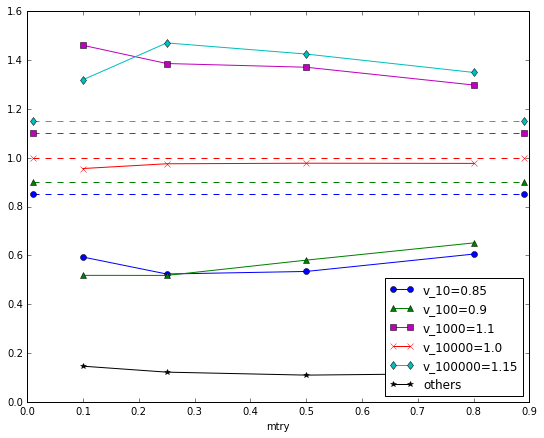
\includegraphics[totalheight=6cm]{./figs/var_oder.png} & 
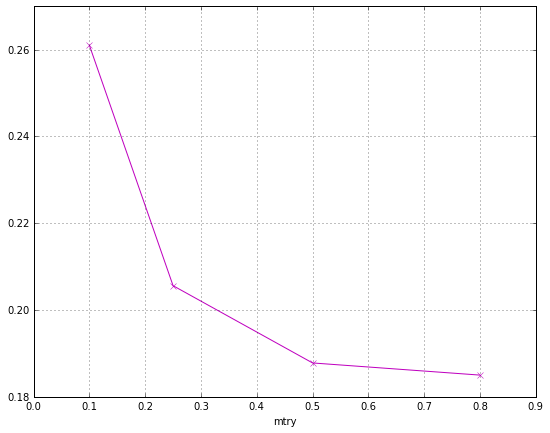
\includegraphics[totalheight=6cm]{./figs/var_oob.png} \\
\end{tabular}
\caption{{\bf Variable importance (Mean Decrease Gini) and OOB (out of bag) classification error estimate for
  random forests with 100 trees trained on the synthetic dataset of 2.5M features and 5K samples.}  {\bf a)} Variable
  importance of top 20 variabels normalized to the sum of the linear model coefficients. {\bf Others} represents
  aggregated importance of variables not present in the linear model.  {\bf b)} OOB (out of bag) classification error
  estimate as funtion of \mtry\ fraction.}
\label{figure:synth}
\end{adjustwidth}
\end{figure}


%%%%%%%%%%%%%%%%%%%%%%%%%%%%%%%%
% Section 2: Feature Selection on real data 
%%%%%%%%%%%%%%%%%%%%%%%%%%%%%%%%
\subsection{\cursedforest\ selects previously demonstrated cancer variants}
%Feature selection can be useful for determining variables the contribute to the label or for perhaps selecting the n most important
%variables for further analysis. 
As established in the pervious section, \cursedforest\ allows the user to retrieve a subsection of features, ranked by
their importance to identify the variables predictive of the label or selecting the $n$ most important variables for
further analysis.  We demonstrate this feature on The Cancer Genome Atlas (TCGA) BRCA dataset.  We build this model on
VCF files retrieved from the TCGA data portal.  For the label, we use the cell type (i.e. tumor or normal).

In Table~\ref{table3}, we display the top 10 features, ranked by their Gini index in the random forest model.

\begin{table}[!ht]
%\begin{adjustwidth}{-2.25in}{0in} % Comment out/remove adjustwidth environment if table fits in text column.
\centering
\caption{
{\bf Features from the TCGA BRCA dataset ranked by their importance.}}
\begin{tabular}{|l|l|l|l|l|l|l|}
\hline
{\bf Variant} & {\bf Gene} & {\bf Importance}\\ \thickhline
x:xxxx & cell2 row 1 & cell3 row 1\\ \hline
x:xxxx & cell2 row 2 & cell3 row 2\\ \hline
x:xxxx & cell2 row 3 & cell3 row 3\\ \hline
\end{tabular}
\begin{flushleft} Here the importance is the gini coefficient when building a model using the cell type as the label.
\end{flushleft}
\label{table3}
%\end{adjustwidth}
\end{table}






%%%%%%%%%%%%%%%%%%%%%%%%%%%%%%%%
% Section 3: Classification selection
%%%%%%%%%%%%%%%%%%%%%%%%%%%%%%%%
\subsection{\cursedforest\ outperforms existing methods for classification problems}
As established in Section~\ref{synthetic}, \cursedforest\ 
In this section we compare \cursedforest 's performance against other published methods for predicting ethnicity on the
1000 Genomes Project dataset.


\begin{table}[!ht]
\begin{minipage}{\textwidth}
\begin{adjustwidth}{-2.25in}{0in} % Comment out/remove adjustwidth environment if table fits in text column.
\centering
\caption{
{\bf Performance comparison between the different machine learning algorithms.}}
\begin{tabular}{|l+l|l|l|l|l|l|p{1cm}|}
\hline
\bf{Genome \%}                      & \bf{Method} & \bf{Error (ARI)} & \bf{Runtime} & \bf{Memory/Node} \\
\hline

\multirow{3}{*}{phase1\_chr22: 1,092 x 490,036} & \cursedforest\ & 0.077 (XX) &                  &                                                                   \\
                                                & RF - Spark ML  &            &                  &                                                                   \\
                                                & RF - R         & 0.05       & 24 min           & 18GB\footnote{using the \texttt{parallel} packages with 10 nodes} \\
                                                & ranger - R      & 0.94       & 1 min 10 seconds & 16GB  (one processor)                                             \\
                                                & ranger - c++     & 0.94       & 7 mins           & --nthreads 20                                                     \\

 \hline
\multirow{3}{*}{phase3\_chr22: 2,504 x 1,103,548}   &               &            &                  &                                                                \\
                                                    & RF - R        & NA         & NA               & NA\footnote{long vectors ($> 2^31-1$)  are not supported in the .Fortran interface} \\
                                                    & H2O           & 0.05       & 16 hours         & 600GB \footnote{java -Xmx600g -jar h2o.jar,   h2o.init(nthreads=20)} \\
                                                    & ranger - R    & 0.94       & 4 1/2 mins       & 21GB (one processor) \\
\hline
\multirow{3}{*}{phase3\_chr1: 2,504 x 6,450,364}    & \cursedforest\ & 0.063 (XX) & 1hr 58min        & 4GB \\
                                                    & RF - Spark ML  & 0.94       & 8hr 29min        & 8GB \\
                                                    & LR - Spark ML  &            & 2hr 6min         & 8GB \\
                                                    & ranger - R      & 0.95       & 28 mins          & num.threads=10\footnote{don't
                                                                                                      know how to get the memory
                                                                                                      used,   This was done on dpas-03} \\
\hline
\multirow{3}{*}{phase3\_chr1-3: 2,504 x 19,328,051} & \cursedforest\ & 0.046 (XX) & 4hr 0min                                             & 4GB \\
                                                    & RF - Spark ML  &            &                                                      & \\
                                                    & LR - Spark ML  &            & 14hr 48min                                           & 8GB \\
                                                    & ranger - R      &  0.97      & 58 mins\footnote{ but took 6 hours to load the
                                                                                   data}
                                                                                                                                         &
                                                                                                                                           909GB\footnote{I
                                                                                                                                           think
                                                                                                                                           this
                                                                                                                                           is
                                                                                                                                           total
                                                                                                                                           memory. The
                                                                                                                                           job
                                                                                                                                           was
                                                                                                                                           run
                                                                                                                                           with
                                                                                                                                                   ntasks-per-node=160
                                                                                                                                           cores-per-socket=10
                                                                                                                                           on
                                                                                                                                           ruby
                                                                                                                                           }  \\
& ranger - R        &             0.973     &      03:58           &       pearcey --cpus-per-task=15 --mem 1600gb   906GB \\
\hline

\multirow{4}{*}{phase3\_chr1-22: 2,504 x 81,047,467} & \cursedforest\ & XX (0.96) & 7hr 14min & 8GB \\
& RF - Spark ML & - & - & - \\
& LR - Spark ML & - & - & - \\ 
& kmeans - Spark ML  & - (0.82)      & 30hr 44min    & 24GB \\ 
& ranger (C++)       &        NA     &        NA     &            80 CPU -- runs out of memory (12.8GB per CPU) \\
& ranger (C++)       &        NA     &        NA     &            160
                                                        CPU -- runs
                                                        out of time at
                                                        20 hours \\
\hline
% \begin{tabular}{|p{1.2cm}|p{1cm}|p{1.5cm}+l|l|p{1.8cm}|p{1.5cm}|}
% \hline
% %\multicolumn{4}{|l|}{\bf Heading1} & \multicolumn{4}{|l|}{\bf Heading2}\\ \hline
% \bf{Data- set} & \bf{Samp- les} & \bf{Feat- ures}  & \bf{Method} & \bf{Error (ARI)} & \bf{Runtime} & \bf{Memory/ Node} \\
% \hline
% %\multirow{3}{*}{phase1\_chr22: 1,092 x 490,036} & CursedForest & 0.077 (XX)  &  &  \\
% phase1 chr22 &1,092 & 490,036 & CursedForest & 0.077 (XX)  & 9min 16sec & 1GB\footnote{\label{note10}10 nodes} \\
% &&& RF - Spark ML & 0.069 (0.89) & 14min 13sec & 1GB\footref{note10}  \\
% &&& RF - R &  0.05  & 24min  & 18GB\footref{note1}\footnote{using the \texttt{parallel} packages}\\
% &&& ranger -R &         0.05 &        1min 10sec  &          16GB  (one processor) \\
%  \hline
% phase3 chr22 & 2,504 & 1,103,548 &  &  &  &  \\
% &&& CursedForest & 0.053 & 9 min 8 sec & 2GB\footnote{\label{note20}20 nodes}\\
% &&& RF - Spark ML & 0.058 (0.92) & 1hr 1min & 2GB\footref{note20} \\
% &&& RF - R & NA  & NA & NA\footnote{long vectors ($> 2^31-1$)  are not supported in the .Fortran interface}\\
% &&&  H2O   &        0.05 &     16 hours       &   600GB \footnote{java -Xmx600g -jar h2o.jar,   h2o.init(nthreads=20)} \\
% \hline
% phase3 chr1 & 2,504 & 6,450,364 & CursedForest & 0.063 (XX) & 1hr 58min & 4GB \\
% &&& RF - Spark ML & (0.94) & 8hr 29min & 8GB \\
% &&& LR - Spark ML&  & 2hr 6min & 8GB\\ 
% &&& ranger  R   &  0.06   &     28 mins  &            num.threads = 10\footnote{don't know how to get the memory used, This
%   was done on dpas-03} \\ 
% \hline
% phase3 chr1-3 & 2,504 & 19,328,051  & CursedForest & 0.046 (XX) & 4hr 0min & 4GB\\
% &&& RF - Spark ML & - & -  & -\\
% &&& LR - Spark ML & & 14hr 48min & 8GB \\ 
% &&& ranger  R   &  0.05   &     58 mins\footnote{ but took 6 hours to load the data}  &      909GB\footnote{I think this is total memory. The job was run with
%   ntasks-per-node=160 cores-per-socket=10 on ruby }  \\ 
% \hline
% phase3 chr1-22 & 2,504 & 81,047,467 & CursedForest & XX (0.96) & 7hr 14min & 8GB \\ 
% &&& RF - Spark ML & - & - & - \\
% &&& LR - Spark ML & - & - & - \\ 
% %&&& kmeans - Spark ML & - (0.82) & 30hr 44min & 24GB \\ 
% \hline
\end{tabular}
\begin{flushleft} 
Comparison of different various machine learning libraries on different subsets of variant data 
from the 1000 Genomes Project.
Each random forest model consists of 50 trees.
\end{flushleft}
\label{table1}
\end{adjustwidth}
\end{minipage}
\end{table}


%%%%%%%%%%%%%%%%%%%%%%%%%%%%%%%%
% Section 4: Sensitivity 
%%%%%%%%%%%%%%%%%%%%%%%%%%%%%%%%
\subsection{Scalability analysis}

In this section we explore the performance of \cursedforest\ by testing its ability to scale to different sizes of data and computational resources.

In order to asses these characteristics we ran \cursedforest\ classification on synthetics datasets with varying numbers of variables (features) and samples, similar to the dataset used in to evaluate ranger [REF: ranger], allocating varying number of CPU cores to the \cursedforest\ and also varying computational complexity of random forests by using range of \mtry\ values.


We investigate the different synthetic datasets generated for section 5.1. and measured the time of building a random forest model of 100 trees and the results reported below are averages of 5 runs. To improve consistency of measurements all the cases were executed with the same random seed.

Firstly we look at CurstedForest horizontal scalability for a medium size dataset of 2.5 million variables and 5000 samples, by varying \mtry\ fraction and the number of CPU cores allocated to the execution. The raw results are presented in the table [REF table1] and visualized in figure [REF: Fig 1] below
Regardless of the number of cores used, \cursedforest\ displays approximately linear dependency between the execution time and the \mtry\ parameter (presented here as a fraction of the number of variables) [Fig 1 a)

\cursedforest\ scales almost linearly with the number of CPU cores for medium values of \mtry\ fraction but for both lower and higher values the performance degrades slightly (Fig 1 b). In the latter case the likely cause is communication overhead (with lower \mtry\ values the proportion of time for parallelizable computation to the time for internode communication is lower) while in the latter case its most likely caused by reaching the clusters computational capacity.

Next we investigate \cursedforest\ scalability with regards to the size of data, by varying the number of variables and sample for a fixed \mtry\ fraction of 0.25 and execution of 128 CPU cores. The raw results are presented in the table [REF] and visualized in figure [ REF: Fig 2] below (please note log scale on the axes and the values on y axes are expresses as trees per hour).

Generally, the number of trees per hour decreases with increased number of variables and samples sizes. Some irregularities in the graph can be attributed to computation vs communication tradeoff. It is also worth noting that keeping \mtry\ fraction constants results with higher \mtry\ values with growing number of variables, and this is what drives the performance down rather that the increase of dataset size itself.


To conclude \cursedforest\ is capable of processing datasets with 50M variables and 10K samples, which is the order of magnitude of the entire genome variants expected in such dataset, for which it can build approximately 60 trees per hour.



\begin{table}[!ht]
\centering
\caption{
{\bf Time in seconds to build a random forest of 100
  trees with specified \mtry\ fraction using given number of CPU cores.}}
\begin{tabular}{|l|l|l|l|l|l|}
\hline
\multicolumn{2}{|l|}{\multirow{2}{*}{}}             & \multicolumn{4}{c|}{Number of CPU cores} \\
\cline{3-6}
\multicolumn{2}{|l|}{}                              & \bf{16} & \bf{32} & \bf{64} & \bf{128} \\
\hline
\multirow{4}{*}{\mtry\ (fraction)}        & \bf{0.10} & 708.3   & 340.0   & 186.0   & 134.5 \\
                                        & \bf{0.25} & 1134.9  & 535.0   & 270.8   & 179.6 \\
                                        & \bf{0.50} & 1724.1  & 856.6   & 428.7   & 243.8 \\
                                        & \bf{0.80} & 2313.5  & 1125.7  & 569.1   & 364.6 \\
\hline
\end{tabular}
\begin{flushleft} 
\end{flushleft}
\label{table10}
\end{table}


\begin{figure}[tbhp]
\begin{adjustwidth}{-1.00in}{0in}
\begin{tabular}{ll}
a)& b)\\
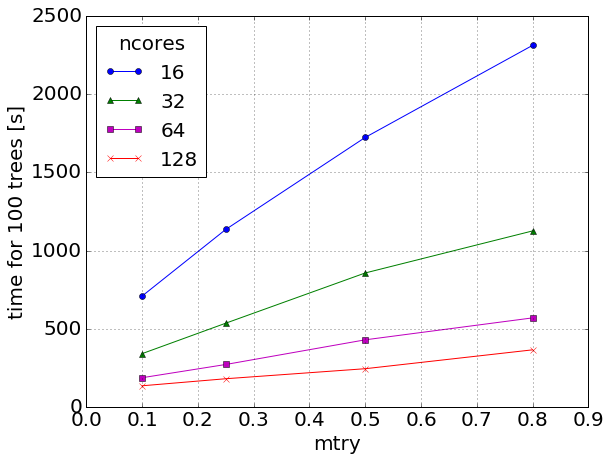
\includegraphics[totalheight=6cm]{./figs/mtry_cpu.png} & 
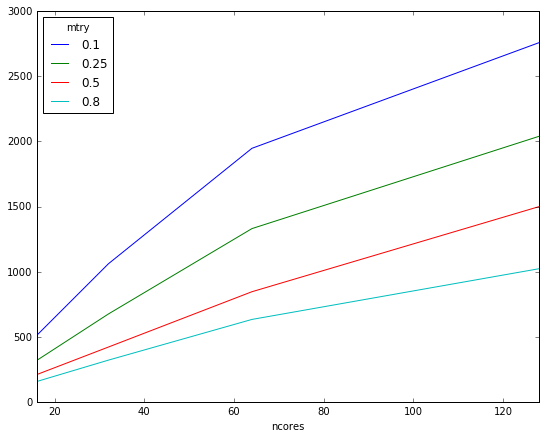
\includegraphics[totalheight=6cm]{./figs/cpu_mtry_trees_per_hour.png} \\
\end{tabular}
\caption{{\bf Scalablity of the wide random forest on the synthetic dataset of 2.5M features and 5K samples.} 
  {\bf a)} Time in seconds to build 100 trees for different \mtry\ fractions. 
  {\bf b)} Number of trees build per hour when using a growing number of CPU cores.}
\label{figure:synth}
\end{adjustwidth}
\end{figure}


%nvars 150000  500000  2500000 10000000  50000000
%nsamples          
%1000  21.6  26.7  59.8  133.5 668.8
%5000  45.7  71.9  186.2 729.3 2887.4
%10000 70.2  120.2 397.3 2237.8  5747.8

\begin{table}[!ht]
\begin{adjustwidth}{-1.00in}{0in}
\centering
\caption{
{\bf Time in seconds to build a random forest of 100
  trees on 128 CPU cores with varying numbers of variables and samples.}}
\begin{tabular}{|l|l|l|l|l|l|l|}
\hline
\multicolumn{2}{|l|}{\multirow{2}{*}{}}           & \multicolumn{5}{c|}{Number of variables} \\
\cline{3-7}
\multicolumn{2}{|l|}{}                               & \bf{150,000} & \bf{500,000} & \bf{2,500,000}  & \bf{10,000,000} & \bf{50,000,000} \\
\hline                                                            
\multirow{4}{*}{Number of samples}      & \bf{1000}  & 21.6  & 26.7  & 59.8  & 133.5  & 668.8 \\
                                        & \bf{5000}  & 45.7  & 71.9  & 186.2 & 729.3  & 2887.4 \\
                                        & \bf{10000} & 70.2  & 120.2 & 397.3 & 2237.8 & 5747.8 \\
\hline
\end{tabular}
\begin{flushleft} 
\end{flushleft}
\label{table10}
\end{adjustwidth}
\end{table}


\begin{figure}[tbhp]
\begin{adjustwidth}{-1.00in}{0in}
\begin{tabular}{ll}
a)& b)\\
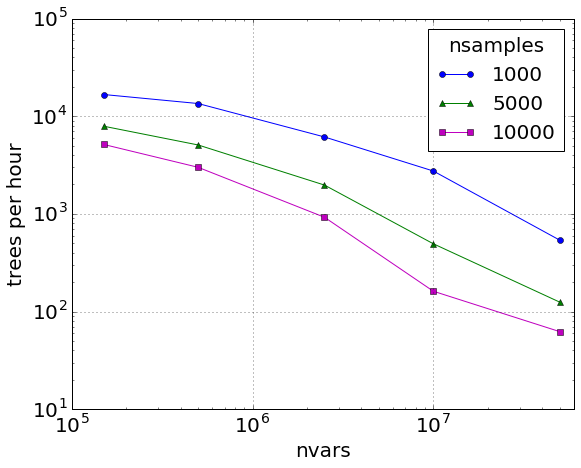
\includegraphics[totalheight=6cm]{./figs/nvars_nsamples.png} & 
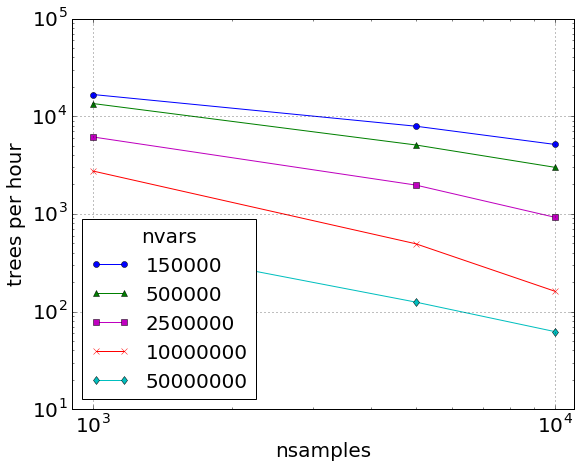
\includegraphics[totalheight=6cm]{./figs/nsamples_nvars.png} \\
\end{tabular}
\caption{{\bf Scalablity of the Wide Random Forest on synthetic datasets with varying number of samples and variables.} 
  {\bf a)} Number of trees build per hour when growing number of variables. 
  {\bf b)} Number of trees build per hour when growing number of samples.}
\label{figure:synth}
\end{adjustwidth}
\end{figure}




\begin{table}[!ht]
\caption{
{\bf Sensitivity analysis on parameter choice.}}
\begin{tabular}{|l|l|l|l|l|l|l|l|}
\hline
%\multicolumn{4}{|l|}{\bf Heading1} & \multicolumn{4}{|l|}{\bf Heading2}\\ \hline
\bf{ \mtry\ }  & \bf{Mtree} & \bf{depth} & \bf{Accuracy} & \bf{Runtime} & \bf{Memory} \\
\hline
&&&&&\\ \hline
\end{tabular}
\begin{flushleft} 
  Table notes here.
\end{flushleft}
\label{table2}
\end{table}




\section{Conclusion}




\section{Supporting Information}

% Include only the SI item label in the subsection heading. Use the \nameref{label} command to cite SI items in the text.
%\subsection*{S1 Video}
%\label{S1_Video}
%{\bf Bold the first sentence.}  Maecenas convallis mauris sit amet sem ultrices gravida. Etiam eget sapien nibh. Sed ac ipsum eget %enim egestas ullamcorper nec euismod ligula. Curabitur fringilla pulvinar lectus consectetur pellentesque.


\section*{Acknowledgments}
Cras egestas velit mauris, eu mollis turpis pellentesque sit amet. Interdum et malesuada fames ac ante ipsum primis in faucibus. Nam id pretium nisi. Sed ac quam id nisi malesuada congue. Sed interdum aliquet augue, at pellentesque quam rhoncus vitae.

\nolinenumbers

\bibliography{./CursedForest.bib}

\end{document}





%  \item D\iaz-Uriarte, R., \& Alvarez de Andr\es, S. (2006). Gene selection and classification of microarray data using random
%    forest. BMC Bioinformatics, 7, 3. http://doi.org/10.1186/1471-2105-7-3
%  \item Goldstein, B. A., Polley, E. C., & Briggs, F. B. S. (2011). Random Forests for Genetic Association Studies. Statistical
%    Applications in Genetics and Molecular Biology, 10(1), 32. http://doi.org/10.2202/1544-6115.1691

%http://stats.stackexchange.com/questions/77018/random-forest-is-it-a-boosting-algorithm
 %http://stats.stackexchange.com/questions/173390/gradient-boosting-tree-vs-random-forest
%overcomes this issue and is hence ideally suited to this application.  Furthermore, random forests are able to capture interactions
%between features, which is of importance for modelling complex polygenic diseases.


% We also investigated classifying the samples using random forests.  We chose random forests due to its ability to
% capture complex interactions between features. Also, due to it being an ensemble method where trees can be formed
% independently, which, is ideal for parallelization. Furthermore, the ensemble of weak learners can help to minimise
% overfitting and variance.



% The reason for the failure can be attributed to the "curse of dimensionality". Where Spark ML is designed to process a
% huge number of samples with a modest dimensionality, the 1000 Genomes data instead contains a huge number of
% dimensions (features). As a result, the default random forests implementation is unable to partition the data into
% small-enough tasks for nodes on the computer cluster to handle.



% For figure citations, please use "Fig." instead of "Figure".
%Nulla mi mi, Fig.~\ref{fig1}  Fusce fringilla erat porttitor lectus cursus, \nameref{S1_Video} vel sagittis arcu lobortis. Aliquam in enim semper, aliquam massa id, cursus neque. Praesent faucibus semper libero.
%\begin{figure}[h]
%\caption{{\bf Figure Title first bold sentence Nulla mi mi, venenatis sed ipsum varius, volutpat euismod diam.}
%Figure Caption Proin rutrum vel massa non gravida. Quisque tempor sem et dignissim rutrum. A: Lorem ipsum dolor sit amet. B: Consectetur adipiscing elit.}
%\label{fig1}
%\end{figure}
%\begin{enumerate}
%\item{react}
%\item{diffuse free particles}
%\item{increment time by dt and go to 1}
%\end{enumerate}

% Results and Discussion can be combined.


%\begin{table}[!ht]
%\begin{adjustwidth}{-2.25in}{0in} % Comment out/remove adjustwidth environment if table fits in text column.
%\caption{
%{\bf Table caption Nulla mi mi, venenatis sed ipsum varius, volutpat euismod diam.}}
%\begin{tabular}{|l|l|l|l|l|l|l|l|}
%\hline
%\multicolumn{4}{|l|}{\bf Heading1} & \multicolumn{4}{|l|}{\bf Heading2}\\ \hline
%$cell1 row1$ & cell2 row 1 & cell3 row 1 & cell4 row 1 & cell5 row 1 & cell6 row 1 & cell7 row 1 & cell8 row 1\\ \hline
%$cell1 row2$ & cell2 row 2 & cell3 row 2 & cell4 row 2 & cell5 row 2 & cell6 row 2 & cell7 row 2 & cell8 row 2\\ \hline
%$cell1 row3$ & cell2 row 3 & cell3 row 3 & cell4 row 3 & cell5 row 3 & cell6 row 3 & cell7 row 3 & cell8 row 3\\ \hline
%\end{tabular}
%\begin{flushleft} Table notes Phasellus venenatis, tortor nec vestibulum mattis, massa tortor interdum felis, nec pellentesque metus tortor nec nisl. Ut ornare mauris tellus, vel dapibus arcu suscipit sed.
%\end{flushleft}
%\label{table1}
%\end{adjustwidth}
%\end{table}
